\chapter{Introduction}

Artificial Intelligence is an extremely interesting but difficult problem to
address, as research has to \emph{at least} account for the complexity and
breath of behaviour that has been shown in animals and humans. Autonomy can
sometimes be programmatically engineered, but most of intelligent behaviour
requires some amount of learning that can only be acquired through direct or
indirect interaction with the environment. A big part of being intelligent has
to do with the ability to generalise knowledge and behave reasonably in unseen
scenarios, which makes formalising and tackling the problem of creating
``intelligence'' a completely unfeasible idea given the great amount of
information humans seem to be able to deal with over their lifetime.

\section{Reinforcement Learning}

A technique developed specifically to solve the problem of learning via
interaction is Reinforcement learning. Reinforcement learning provides a general
framework in which to learn behaviour in a goal-oriented fashion and without
requiring expert knowledge or labelled data \citep{Sutton:1998:IRL:551283}. It
is framed to be functional in non-deterministic environments and even in
situations where reward is extremely delayed. Because of its foundations on
dynamic programming and control theory, algorithms framed around the
reinforcement learning setting can ultimately be analysed using a rich set of
powerful mathematical tools \citep{puterman1990markov,beard1997galerkin}.
Unfortunately those algorithms learn relatively good behaviour only when the
decision-making problem is tractable, that is when the environment is both
sufficiently representable and observable \citep{kaelbling1996reinforcement};
moreover reinforcement Learning algorithms also tend to break down as the state
space increases in size and dimensions \citep{doya2000reinforcement}. To study
and improve those algorithms we therefore need testbeds that provide facilities
to parametrise the size of the state and the general difficulty of the task,
while remaining interesting enough to provide challenges for evolving
state-of-the-art algorithms.

\section{Games as Virtual Learning Environments}

Reinforcement Learning algorithms have since the beginning found usage when
applied to fields such as robot control, natural language processing and
economics, but most of the theoretical work has required the usage of relatively
simple and scalable testbeds to develop and compare algorithms in a systematic
and rigorous manner. Most of those domains consisted in direct adaptations of
classical AI problems such as grid worlds and bandit problems, but as research
started getting past those simple domains the community had to come up with more
structured and complex environments. 

The idea of using games as testing framework for Artificial Intelligence is
certainly not a new one. Chess, Backgammon, Go and various other board games
have historically been linked to challenges and advances in AI research
\citep{minsky1961steps}, and the AI community has often used those games to
compare and study the properties of different algorithms
\citep{silver2009reinforcement, tesauro1995temporal, campbell2002deep}.

Over the past couple of decades researchers have gradually started to solve or
fully tackling most of those board games, leaving themselves and their
colleagues with fewer available platforms and generally too large domains to
make gradual reinforcement learning research easily achievable. On the other
hand, computer games have always provided the community a perfect excuse to
study search algorithms and symbolic solvers because of the need to challenge
human players, allowing at least part of the community to steadily keep working.

\begin{figure}[h]
    \centering
    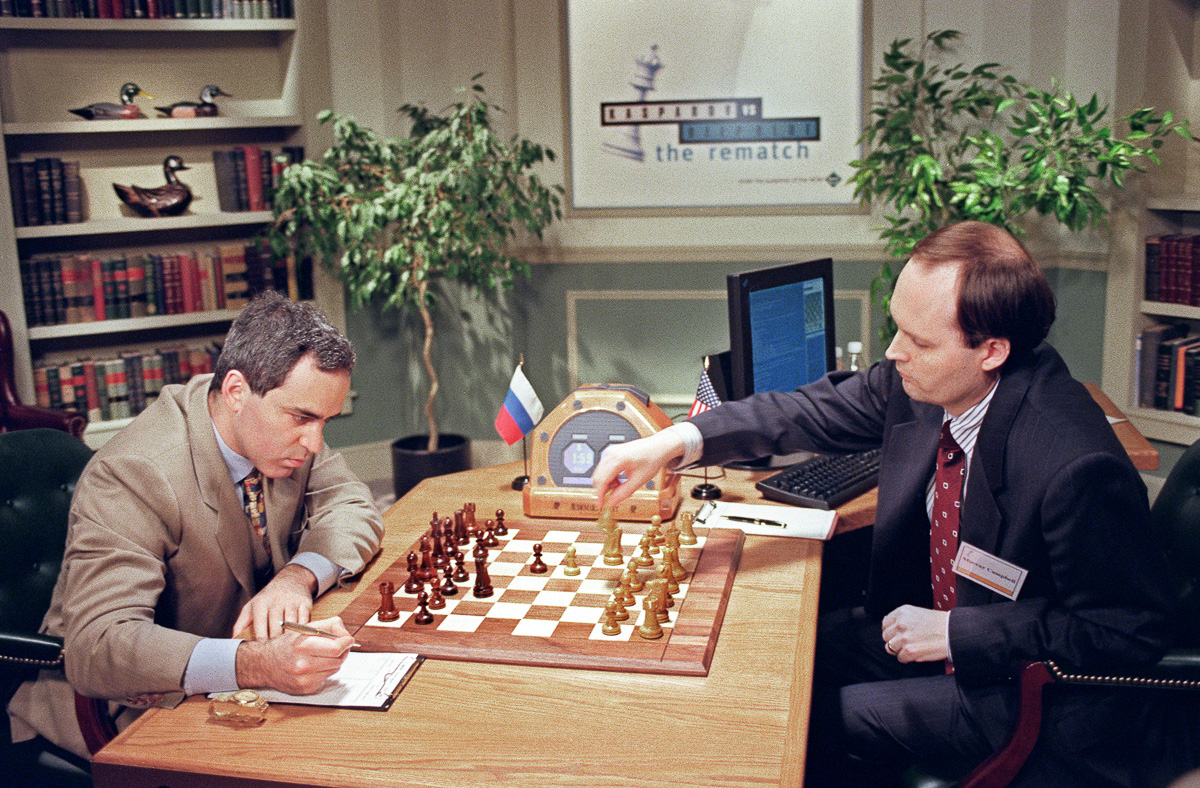
\includegraphics[width=0.9\textwidth]{ch1/kasparovdeepblue}
    \caption{May 1997: IBM scientist Murray Campbell makes a move for Deep Blue
      in the second game of the historical match. (Image: Stan Honda / AFP /
      Getty Images)}
    \label{fig:kasparovdeepblue}
    % see http://mashable.com/2016/02/10/kasparov-deep-blue/#CisvTzeeqkqV
\end{figure}

Recently other domains such as football \citep{kitano1997robocup}, simulated car
racing \citep{wymann2013torcs} and a variety of computer games also started
gaining popularity as suitable platforms for research in decision making. All of
those share characteristics that make naive reinforcement learning complex to
engineer and use: they possess large action or environment state spaces, they
challenge algorithms by providing a degree of partial observability, or they can
often be properly tackled only with the involvement of strong long-term
strategies (with complexity more suitable for communities working on long-term
planning).

\begin{figure}[h]
    \centering
    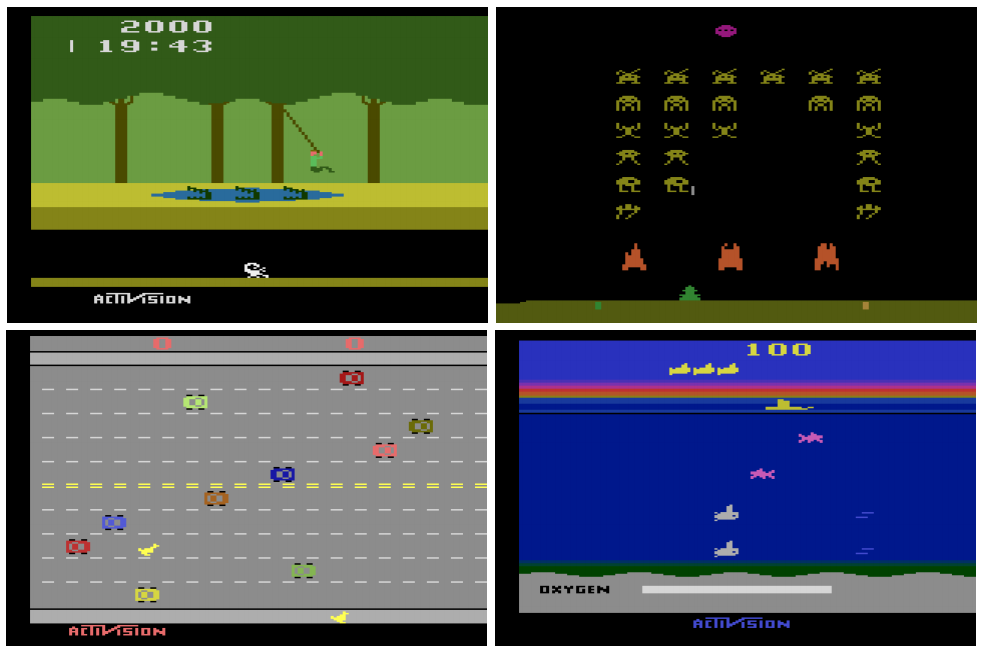
\includegraphics[width=0.9\textwidth]{ch1/ale}
    \caption{Screenshots of some of the games available within the Arcade
      Learning Environment. Clockwise from top-left: Pitfall!, Space Invaders,
      Freeway, and Seaquest.}
    \label{fig:ALE}
\end{figure}

An example of such recent and popular learning platform is the Arcade Learning
Environment (ALE) \citep{bellemare2012arcade}, which researchers have mostly
used to study reinforcement learning algorithms that can learn a variety of
policies for different games of various complexity. Unfortunately the majority
of the games contained in this particular platform don't necessarily require
anything way more complex than reactive policies, which means that studying more
advanced learning tasks on those games has recently become quite a forced
process.

A category of computer games instead more suitable for providing complex
scenarios for studying RL is the category of Real-Time Strategy (RTS) games.
This typology of games generally requires some amount of long-term planning
combined with interactive and generalisable short-term (and reactive)
decision-making, with the complexity becoming almost entirely context-dependent,
(as it is often the case in real-life scenarios). Those are particularly
challenging to existing classical reinforcement learning algorithms because of
the often intrinsic partial observability, the unusually big action space, and
their nature of competitive game which makes modelling adversarial processes
almost a requirement. In this thesis we focus on one of the most popular and
still widely played RTS games, \emph{StarCraft: Brood War}.

% TODO maybe cite from
% http://umichrl.pbworks.com/w/page/7597597/Successes%20of%20Reinforcement%20Learning

\section{Thesis Work}

This work focused primarily on exploring what it would take to concretely
transform and use StarCraft as a platform to study reinforcement learning and
general artificial intelligence. We adopted a scoping approach to deal with the
engineering problem, with the goal to reach a state where we could successfully
run state of the art learning algorithms using the game as the environment. This
led us to the design and development of a robust and generic framework based on
\emph{StarCraft: Brood War}, to the creation of an interface to Torch (one of
the most popular currently available tensor libraries), and finally to port and
test a few variations of commonly used reinforcement learning and deep
reinforcement learning algorithms.

The idea was to prove the feasibility of using StarCraft as a learning platform,
to release the first version of a useful interface to allow the community to
bootstrap work on real-time strategy games, and to create a baseline for later
work in the area.

\section{Report Structure}

Chapter 2 presents the reinforcement learning framework and discusses some of
the research based on computer games. We outline properties of Real-Time
Strategy games, and we seek to explain the benefits of using StarCraft as a
research platform. Chapter 3 presents the engineering approach taken and the
developed architecture, covering the entire pipeline from the game to the agent
interface. Chapter 4 provides a description of our testing tasks and the design
and implementation of our reinforcement learning algorithms. Chapter 5 outlines
results obtained from empirically testing the framework and analysing the
performances of the agents on our task. Finally Chapter 6 gives a critique of
our work and discusses some possible improvements, delineating some future work
we already started developing.
